\chapter{Схема электрической коммутации компонентов 3D-принтера}\label{app:commutation_scheme}

Наглядная схема электрической коммутации компонентов принтера приведена на рисунке~\ref{fig:appendix_commutation_scheme}.

\begin{figure}[h!]
\begin{center}
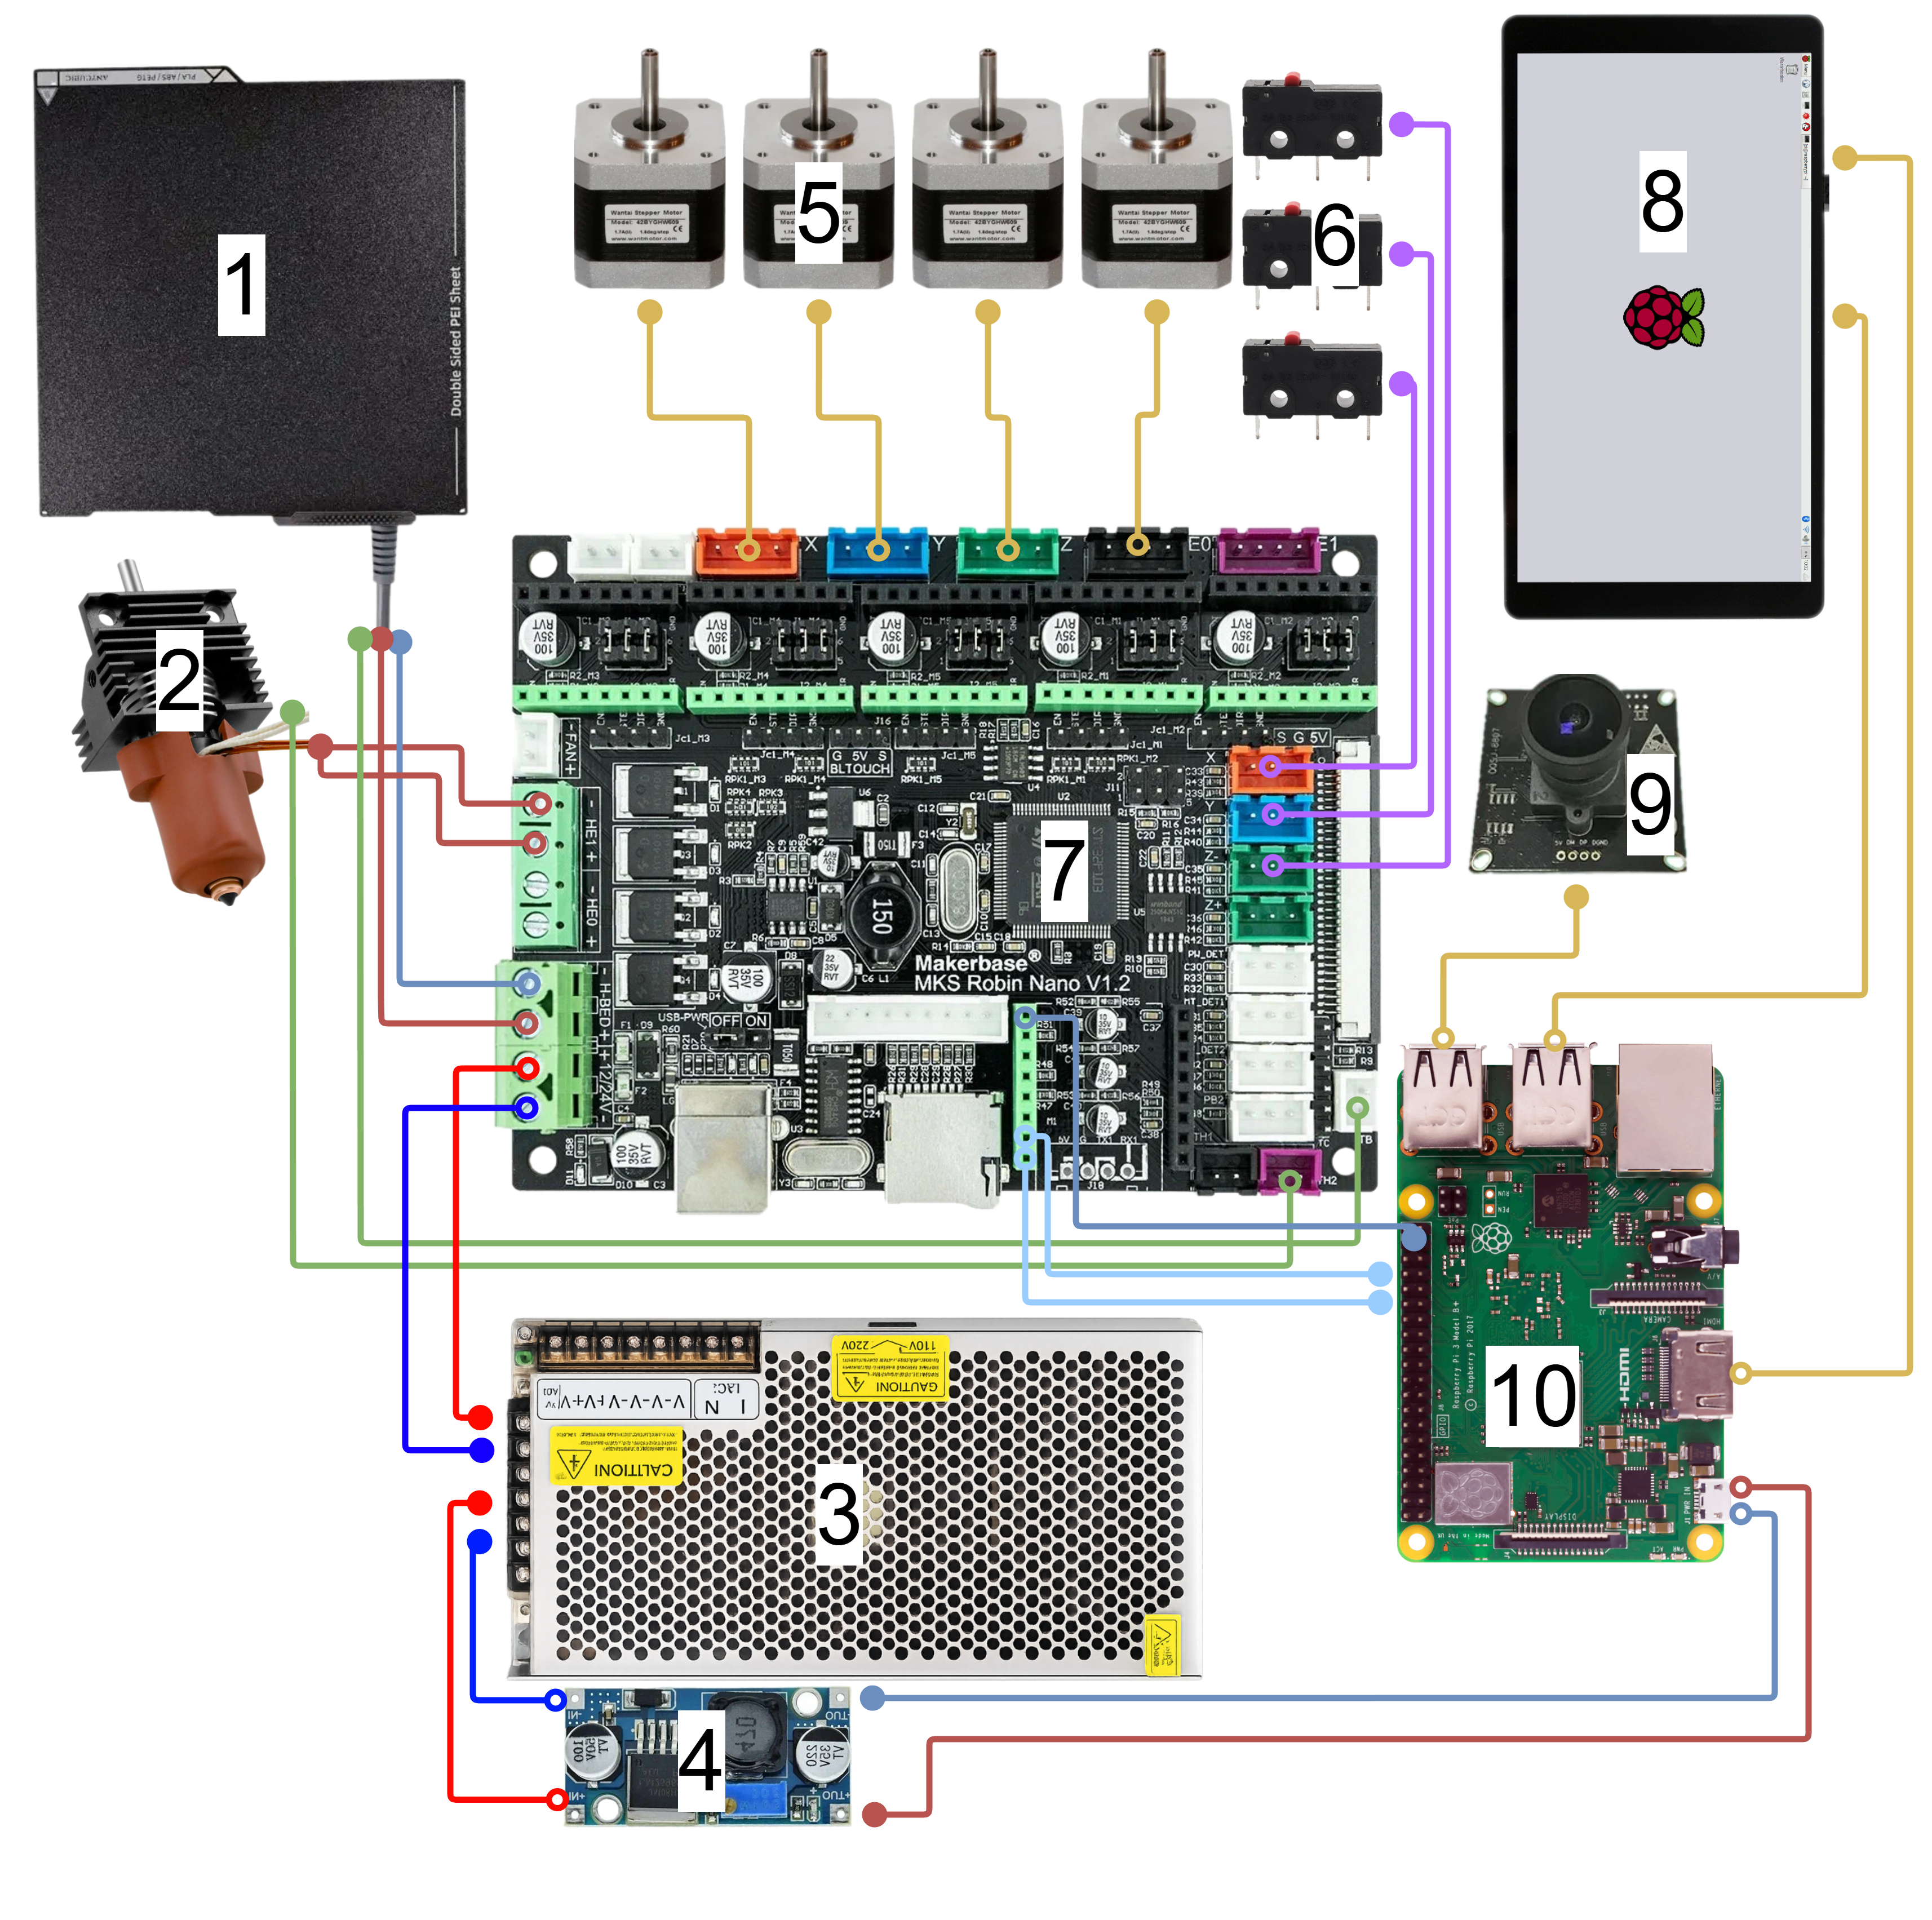
\includegraphics[width=\hsize]{fig/commutation_diagram_nir2.png}
\caption{Схема электрической коммутации компонентов 3D-принтера}\label{fig:appendix_commutation_scheme}
\end{center}
\end{figure}

Описание подключений по позициям схемы:

\begin{itemize}
\item Позиция 1 — нагреваемый стол. Нагревательный стол подключается к плате MKS Robin Nano~1.2 как силовая нагрузка контура стола. В актуальной конфигурации прошивки это соответствует блоку \texttt{[heater\_bed]} с каналом управления нагревом \texttt{heater\_pin: PA0}. Температурный контроль стола реализован через отдельный термодатчик, подключенный к измерительному входу платы; в профиле задано \texttt{sensor\_type: NTC100K\_B3950} и \texttt{sensor\_pin: PC0}. Для безопасной эксплуатации заданы программные ограничения и проверка набора температуры (\texttt{max\_temp: 120}, \texttt{max\_power: 1.00}, блок \texttt{[verify\_heater heater\_bed]}).

\item Позиция 2 — нагреватель и термистор хотэнда. Нагреватель хотэнда подключен к плате MKS Robin Nano~1.2 как отдельный силовой канал экструдера; в актуальном профиле это блок \texttt{[extruder]} с \texttt{heater\_pin: PB0}. Термодатчик хотэнда подключен к отдельному измерительному входу платы и описан как \texttt{sensor\_type: NTC100K\_B3950} с \texttt{sensor\_pin: PC1}. Для защиты от нештатных режимов заданы температурные и технологические ограничения (\texttt{max\_temp: 280}, \texttt{max\_power: 1.0}, \texttt{min\_extrude\_temp: 170}).

\item Позиция 3 — блок питания. Блок питания работает от сети 220~В и формирует выходную шину 24~В для низковольтной части принтера. В данной конфигурации напрямую к выходу блока питания подключены только плата MKS Robin Nano~1.2 и понижающий преобразователь DC-DC. Подключение остальных нагрузок выполняется через плату MKS.

\item Позиция 4 — понижающий преобразователь DC-DC. Понижающий преобразователь получает питание от шины 24~В и формирует стабилизированную линию 5~В для низковольтной подсистемы. К выходу преобразователя подключены Raspberry Pi~3B, USB-камера Sonix USB 2.0 и экран. Такое разделение контуров позволяет питать хостовые устройства от отдельной линии 5~В и не подключать их напрямую к выходам платы MKS Robin Nano~1.2.

\item Позиция 5 — шаговые двигатели и драйверы TMC2209. Подключение двигателей выполнено через моторные разъемы платы MKS Robin Nano~1.2, обозначенные в даташите как \texttt{X}, \texttt{Y}, \texttt{Z1}, \texttt{E0}, \texttt{E1}. В текущей конфигурации задействованы \texttt{X}, \texttt{Y}, \texttt{Z1} и \texttt{E0}; разъем \texttt{E1} не используется. Для этих каналов установлены драйверы TMC2209, при этом в профиле прошивки задано \texttt{microsteps: 16}, а секции \texttt{[tmc*]} отсутствуют, что соответствует автономному режиму работы драйверов.

\item Позиция 6 — концевые выключатели. Концевые выключатели осей X, Y и Z подключены к сигнальным входам платы MKS Robin Nano~1.2 и используются для выполнения процедуры фиксации базовых координат принтера. В профиле прошивки они заданы как \texttt{endstop\_pin: \^PA15} для оси X, \texttt{endstop\_pin: \^PA12} для оси Y и \texttt{endstop\_pin: \^PA11} для оси Z. Корректная работа концевых выключателей влияет на точность базирования и предотвращает выход механики за допустимые пределы перемещения.

\item Позиция 7 — плата управления MKS Robin Nano~1.2. Плата является центральным узлом коммутации и управления: на нее подается питание 24~В, к ней подключаются исполнительные и измерительные цепи принтера, а также линия связи с Raspberry Pi. На уровне прошивки MKS работает как MCU в контуре Klipper, выполняя обработку команд реального времени для двигателей, нагревателей и датчиков. В текущей конфигурации обмен с хостом выполняется по UART, что соответствует принятой архитектуре управления в проекте.

\item Позиция 8 — AMOLED-экран. Экран подключен к Raspberry Pi по интерфейсу HDMI для вывода изображения и по USB для работы сенсорного ввода. Такая схема разделяет видеоканал и канал передачи событий касания, что обеспечивает корректную работу локального интерфейса управления.

\item Позиция 9 — камера. Камера подключена к Raspberry Pi по USB и используется как источник видеоданных для наблюдения за зоной печати. Далее видеопоток передается в программный контур мониторинга и используется для обнаружения отклонений в процессе 3D-печати.

\item Позиция 10 — Raspberry Pi~3B. Raspberry Pi является хост-узлом контура управления: на нем работают сервисы Klipper и Moonraker, а также подсистема видеомониторинга. Сигнальная связь с платой MKS Robin Nano~1.2 выполнена по UART через контактный разъем GPIO Raspberry Pi и разъем WiFi-UART платы MKS: \texttt{GPIO14 / pin 8 (TX) -> PA10 (RX)}, \texttt{GPIO15 / pin 10 (RX) -> PA9 (TX)}, общий провод \texttt{GND -> GND}. В текущей конфигурации проекта именно этот UART-канал используется как основной рабочий канал связи.
\end{itemize}

\chapter{Последовательность этапов сценария развертывания}\label{app:loader_steps}

В данном приложении приведен полный перечень шагов shell-сценария \texttt{loader.sh}, используемого для воспроизводимого развертывания программного контура в репозитории \texttt{treed-mainshellOS}. В рамках сценария используются два типа этапов: \texttt{required} (ошибка прерывает процесс) и \texttt{optional} (ошибка фиксируется в журнале, после чего выполнение продолжается). Под развертыванием в данном контексте понимается автоматизированная подготовка системы к рабочему состоянию, включая настройку загрузки, сервисов и runtime-конфигурации печати.

\begin{enumerate}
\item \texttt{check-env.sh} --- выполняет базовую валидацию окружения запуска: проверяет права, обязательные переменные контракта лоадера и доступность целевого домашнего каталога пользователя.
\item \texttt{detect-rpi.sh} --- определяет модель Raspberry Pi и реальные boot-пути, после чего экспортирует их для последующих шагов, чтобы исключить расхождения между вариантами разметки boot-раздела.
\item \texttt{timezone-sync.sh} --- синхронизирует часовой пояс и состояние службы времени по протоколу Network Time Protocol (NTP), что требуется для корректной временной метки логов и событий.
\item \texttt{maintenance-stop.sh} --- переводит систему в режим обслуживания: останавливает ключевые runtime-сервисы перед изменением конфигурации и предотвращает конфликты доступа к файлам.
\item \texttt{packages-core.sh} --- устанавливает базовые системные зависимости и выполняет санитарные проверки критичных утилит, которые используются в последующих этапах сценария.
\item \texttt{boot-hdmi-config.sh} --- приводит к целевому виду блок настроек видеовыхода High-Definition Multimedia Interface (HDMI) и параметр \texttt{gpu\_mem} в \texttt{config.txt}, сохраняя управляемую и идемпотентную структуру файла.
\item \texttt{rpi-uart-config.sh} --- подготавливает канал Universal Asynchronous Receiver-Transmitter (UART) для связи с микроконтроллерным узлом (MCU): нормализует \texttt{enable\_uart}, отключает конфликтующую serial-console и применяет правила доступа к UART-устройствам.
\item \texttt{plymouth-theme-install.sh} --- устанавливает тему Plymouth (подсистема графической заставки загрузки Linux), проверяет полноту ее файлов и назначает тему по умолчанию.
\item \texttt{plymouth-initramfs.sh} --- пересобирает \texttt{initramfs} (образ ранней инициализации Linux) с установленной темой загрузки и копирует актуальный образ в boot-раздел.
\item \texttt{plymouth-initramfs-config.sh} --- вносит в \texttt{config.txt} согласованную строку подключения \texttt{initramfs} и отключает конфликтующие автоматические механизмы при их наличии.
\item \texttt{plymouth-cmdline.sh} --- нормализует параметры kernel command line (\texttt{cmdline}), удаляет конфликтные токены и формирует целевой набор параметров загрузки в фиксированном порядке.
\item \texttt{plymouth-systemd.sh} --- согласует состояние systemd-юнитов, связанных с консолью и завершением заставки загрузки, чтобы поведение при старте системы оставалось предсказуемым.
\item \texttt{klipper-sync.sh} --- синхронизирует дерево конфигураций Klipper из репозитория в промежуточный каталог (\texttt{staging}) с нормализацией владельца файлов.
\item \texttt{klipper-profiles.sh} --- применяет профиль RN12 и вычисляет корректный serial-путь MCU для выбранного транспорта (\texttt{usb} или \texttt{uart}), после чего идемпотентно обновляет \texttt{mcu\_rn12.cfg}.
\item \texttt{klipper-core.sh} --- переносит конфигурацию из \texttt{staging} в рабочий каталог (\texttt{runtime}), учитывая режим развертывания (\texttt{clean} или \texttt{preserve}) и сохранение локальных переопределений при необходимости.
\item \texttt{klipper-anti-shutdown.sh} --- диагностирует состояние Klipper после раскладки и при обнаружении аварийного состояния MCU выполняет контролируемый \texttt{FIRMWARE\_RESTART}.
\item \texttt{moonraker-config.sh} --- развертывает конфигурацию Moonraker (API-сервис взаимодействия с Klipper), выполняет валидацию и перезапуск с проверкой готовности сервиса.
\item \texttt{crowsnest-webcam.sh} (\texttt{optional}) --- настраивает видеоконтур через crowsnest (служба публикации потока камеры), подготавливает webcam-фрагменты конфигурации и выполняет проверки доступности устройства.
\item \texttt{treed-cam.sh} --- разворачивает runtime-скрипты камерного контура TreeD, нормализует права и исполняемость shell-файлов для дальнейшего использования в рабочем цикле.
\item \texttt{klipper-mainsail-theme.sh} --- выполняет синхронизацию темы пользовательского интерфейса Mainsail в runtime-конфигурацию.
\item \texttt{klipperscreen-install.sh} (\texttt{optional}) --- устанавливает и проводит первичную проверку KlipperScreen (локальный экранный интерфейс управления принтером).
\item \texttt{klipperscreen-theme.sh} (\texttt{optional}) --- разворачивает тему, шрифты и параметры языка для KlipperScreen, после чего перезапускает сервис для применения изменений.
\item \texttt{klipperscreen-integr.sh} (\texttt{optional}) --- применяет systemd override для корректной интеграции KlipperScreen в цепочку запуска и проверяет успешность перезапуска.
\item \texttt{maintenance-start.sh} --- завершает режим обслуживания и запускает required/best-effort сервисы с ожиданием перехода в рабочее состояние.
\item \texttt{verify.sh} --- выполняет финальную валидацию всего контура: проверяет boot-настройки, сервисы, serial-путь MCU, параметры UART/USB, состояние камеры и формирует итог pass/fail по результатам проверок.
\end{enumerate}
